This chapter will focus on the main probabilistic knowledge necessary to have a strong mathematical base. One of the key thing to know about
probabilities is that all the theory is builded from the set theory. Because of that the very first points to take into account will be the
fundamental set aspects. After that the chapter will go inside into the probabilistic theory.

\section{Set Theory}
Informally, a set can be defined as a collection of objects. The formally definition of what it's a set vary depending of the axiomatic definition
of choice. Because set theory is not into the aim of this book and because sets can be studied intuitively, we are going to refer to it in his more 
fundamental form. Venn diagrams can be used to understand graphically most of the properties of sets.

\subsection{Notation}
If an object $o$ is an element of a set $A$, then we can write $o \in A$. A set and his elements can be denoted by
\begin{center}
    $A = \{o_1, o_2, \dots , o_n\}$ where $n$ can be \textit{finite} or \textit{infinite}
\end{center}
If all elements of a set $B$ are also member of a set $A$ then we can say that $B$ is a subset of $A$ and it's denoted by $B \subset A$ or $B \subseteq A$ 
if $A$ and $B$ has exactly the same elements.\\
Sometimes a especial set $U$ is used to refer the set that contains all possible objects.

\subsection{Binary Operations}
Set theory defines a group of operations that can be performed between two sets. Some of them are:
\begin{itemize}
    \item \textbf{Union} of $A$ and $B$, denoted $A \cup B$, is the set of all objects that are a member of $A$, or $B$, or both.
    \item \textbf{Intersection} of $A$ and $B$, denoted $A \cap B$, is the set of all objects that are members of both $A$ and $B$.
    \item \textbf{Complement} of $A$ refers to elements not contained in $A$. Denoted $\overline{A}$ or $A^c$
    \item \textbf{Difference} of $A$ and $B$, denoted $A \setminus B$, is the set of all members of $A$ that are not members of $B$
    \item \textbf{Power} of $A$, denoted $\mathcal{P}(A)$, is the set whose members are all of the possible subsets of $A$. 
\end{itemize}

\subsection{Properties}
Derived from above there is some general properties called the \textbf{fundamental properties of set algebra}. These properties 
are essential to understand the set theory. In fact, if the set theory is completely understand, these properties are automatically 
assimilated. Thus it's not necessary to memorize it. 
\begin{itemize}
   \item Commutative: 
   \begin{itemize}
        \item[] $A \cup B = B \cup A$
        \item[] $A \cap B = B \cap A$
   \end{itemize}
   \item Associative: 
   \begin{itemize}
        \item[] $(A \cup B) \cup C = A \cup (B \cup C)$
        \item[] $(A \cap B) \cap C = A \cap (B \cap C)$
   \end{itemize}
   \item Distributive:
   \begin{itemize}
        \item[] Union with Intersection: $(A \cap B)\cup C = (A\cup C) \cap (B \cup C) $
        \item[] Intersection with Union: $(A \cup B)\cap C = (A\cap C) \cup (B \cup C) $
   \end{itemize}   
   \item Neutral Element: $A \cup \emptyset = A = A \cap S$
   \item Complementation: $A \cup \overline{A} = S$ and $A\cap \overline{A} = \emptyset$
   \item Idempotence: $A \cup A = A$ and $A \cap A = A$
   \item Abosortion: $A \cup S = S$ and $A \cap \emptyset = \emptyset$
   \item Simplication: $A \cap (A \cup B) = A = A \cup (A \cap B)$
\end{itemize}

\textbf{De Morgan's laws}
\begin{itemize}
   \item $\overline{A \cup B} = \overline{A} \cap \overline{B}$
   \item $\overline{A \cap B} = \overline{A} \cup \overline{B}$
\end{itemize}

\section{Combinatory}
Also know as expertise in counting

\subsection{Rule of Product}
If there are $\alpha$ ways of doing something and $\beta$ ways of doing another thing, then there are $\alpha\beta$ ways of performing both actions.

\subsection{k-permutations}
\textbf{k-permutations of n elements:}\\
The number of \textbf{ordered sequences} with $1\leq k \leq n$ that can be formed of $n$ elements is,
\[ n(n-1)(n-2)\dots(n-k+1) = \frac{n!}{(n-k)!} \]

\subsection{k-combinations}
\textbf{k-combinations of n objects:}\\
The number of \textbf{unordered sequences} within a set with $1\leq k \leq n$ that can be formed of $n$ elements is,
\[ \binom{n}{k} = \frac{n!}{k!(n-k)!} \]

\subsection{Partitions}
$r$ groups containing $n_i$ objects each,
\[ \binom{n}{n_1,n_2\dots,n_r} = \frac{n!}{n_1!n_2!\dots n_r!} \]

\section{Random Experiments}
 A experiment is deterministic when knowing the state of the set of variables involved in the experiment the outcome is always the same.
 Conversely a experiment is random when knowing the state (or when we ignore some of these states) of the set of variables involved in
 the experiment the outcome differs. \\
 
 In other terms, \textbf{an experiment is random} if although it is repeated in the same manner every time, can result in different outcomes. 
 Thus, the fixed outcome of a random experiment is impossible to predict in advance although the number of individual possibles outcomes is known in 
 advance.
 The probability theory study the random experiments.\\

 The notation of some elements involved in a random experiment are the followings:
 \begin{itemize}
     \item \textbf{Sample Space}, is the set of all possible outcomes of the random experiment. It's denoted by $S$ or $\Omega$
     \item \textbf{Individual Outcomes}, are the type of possible outcomes of a random experiment. It's denoted by $\omega$
     \item \textbf{Event}, is a subset of $S$. Usually denoted by capital letters starting by $A$, $B$, $C$, etc. 
        Sometimes denoted by $\mathcal{F}$ for his general form. 
     \item \textbf{Null Event}, is a special event that never occurs. Denoted by $\emptyset$
     \item \textbf{Frequency} of $\omega$ is the number of times the individual outcome $\omega$ occurs in a random experiment.
     \item \textbf{Relative Frequency} of $\omega$ is the ratio between the frequency of $\omega$ and the total number of outcomes of a random experiment.
 \end{itemize}

 Once the experiment has been performed, it is said that $A$ “happened” if the outcome of the experiment ( $\omega$ ) belongs to $A$. 

 \subsection{Events Operations}
If the logical meaning from the set operations is taken and restricted to a probabilistic perspective, then a new meaning for these operations can be defined
in this new scope. Thus:
\begin{itemize}
    \item \textbf{Union} $A \cup B$ (Grammatically $A$ or $B$), occurs when either of the two events (or both of them simultaneously) do occur.
    \item \textbf{Intersection} $A \cap B$ (Grammatically $A$ and $B$), occurs when both of them do simultaneously occur.
    \item \textbf{Complementary} $\overline{A}$ (Grammatically not $A$), occurs when the event does not occur.
    \item \textbf{Difference} $A \setminus B$ (Grammatically $A$ and not $B$), occurs when the first event does occurs, but the second does not. 
                Note that $A \setminus B = A \cap \overline{B}$
\end{itemize}

\subsection{Formal Definitions}
From an formal perspective, the concept of probability has been defined multiples times. Here they are collected the fundamental ones that tries
to formalize the abstract concepts of what it's usually understand as probability and his parts.

\subsubsection{$\sigma$-algebra}
A $\sigma$-algebra (sigma-algebra) $\mathcal{A}$ over a set $\Omega$ is a family (collection) of subsets (with elements $E_1, E_2, \dots$) of $\Omega$ that satisfies:
\begin{itemize}
    \item $\emptyset \in \mathcal{A}$
    \item If $E \in \mathcal{A}$ then $\overline{E} \in \mathcal{A}$
    \item If $E_1, E_2, \dots \in \mathcal{A}$ then $\cup_{n=1}^{\infty}E_i \in \mathcal{A}$ 
\end{itemize} 

\subsubsection{$\sigma$-algebra discrete} 
The discrete $\sigma$-algebra of $\Omega$ is the power set of $\Omega$ ($\mathcal{P}(\Omega)=\{E : E \subset \Omega\}$), that is, the collection
of all subsets of $\Omega$.\\

\textbf{For example,} given a random experiment that toss one coin,
\begin{itemize}
    \item[] $H$: The coin shows head.
    \item[] $T$: The coin shows tail. 
    \item[] $S = \{H, T\},\;\;\; \mathcal{P}(S)=\{\emptyset, \{H\}, \{T\}, S\}$
\end{itemize}

\subsubsection{Measurable Space}
The pair $(\Omega, \mathcal{A})$ is a measurable space if $\mathcal{A}$ is a $\sigma$-algebra over $\Omega$

\subsubsection{Frequentist Definition}
The probability of an event $A$ is the limit of the relative frequency of that event when the number of repetitions of the experiment tends to infinity.
If the experiment is repeated $n$ times, and $n_A$ is the number of repetitions in which $A$ happens, then the probability of $A$ is
\[ P(A) = \lim_{n \rightarrow \infty} \frac{n_A}{n} \] 

\subsubsection{LaPlace's Definition}
This definition can be used for random experiments that have a finite number of outcomes and all of them are equally likely.\\
The probability of an event $A$ is the ratio between the favorable outcomes to $A$ and the total outcomes of the experiment, thus,
\[  P(A) = \frac{\#A}{\#\Omega}  \]

This implies that, given,
\[ S = \{s_1,s_2,\dots\, s_n\},\;\;\; P(s_n)=\frac{1}{n} \]

\subsubsection{Kolmogorov Definition}
The Kolmogorov definition is the only one that does not define what is a probability function. In fact, this definition stablish three axioms that must be
satisfied by any probability function. This axioms are a fundamental part of probability theory.\\
Let the pair $(\Omega, \mathcal{A})$ be a \textit{measurable space}. In it, the probability function $P$ of some event $E$, denoted $P(E)$ is an application
over the real numbers ($P: \mathcal{A} \rightarrow \mathbb{R}$) that satisfies:

\begin{itemize}
    \item \textbf{Non Negativity}: $P(E) \geq 0, \forall E \in \mathcal{A}$
    \item \textbf{Unitarity}: $P(\Omega) = 1$
    \item \textbf{Additivity}: Any countable sequence $E_1, E_2, \dots$ of disjoint events of $\mathcal{A}$, satisfies
            \[ P(\bigcup_{n=1} E_i) = \sum_{n=1} P(E_i) \]
\end{itemize}

\subsubsection{Cox's Theorem}
Used by bayesians. TODO

\subsection{Properties}
These are the properties that apply independency of the probability definition of choice.
\begin{itemize}
    \item $P(\overline{A}) = 1 - P(A)$
    \item $P(\emptyset) = 0$
    \item If $A \subseteq B$ then $P(A) \leq P(B)$
    \item $P(A\setminus B) = P(A) - P(A \cap B)$
    \item $P(A \cup B) = P(A) + P(B) - P(A \cap B)$
    \item $P(A \cup B \cup C) = P(A \cup (B \cup C)) = P(A) + P(B) + P(C) + P(A\cap B \cap C) - P(A \cap B) - P(A \cap C) - P(B \cap C)$
\end{itemize}

\subsection{Conditional Probability}
The probability of the event $A$ occurs knowing before hand that the event $B$ has occurred is,
\[  P(A|B) = \frac{P(A\cap B)}{P(B)} \]
Note that when we have a conditional probability, it can be say that $B$ becomes the new sample space of the experiment.

\subsubsection{Properties}
The conditional probability holds all the properties of the regular probability.

\subsection{Bayes Theorem}
Given a set of events $A_1, A_2, \dots, A_n$, the probability of all of them occurring simultaneously is called \textbf{probability chain rule}, and it is
\[ P(A_1\cap A_2 \cap \dots \cap A_n) = P(A_1)P(A_2|A_1)\dots P(A_n|A_1\cap \dots \cap A_{n-1}) = \prod_{k=1}^{n}P(A_k|\bigcap_{j=1}^{k-1}A_j) \]
or alternatively, in his two events form,
\[ P(A \cap B) = P(A)P(B|A)\]

\subsubsection{Total Probability Rule}
Given $A_1,\dots,A_n$ mutually exclusive (disjoint) events whose union is the whole of the sample space (partition) and assume $P(A_i) > 0$ for every $i$ .For every 
event $B$ we have
\[ P(B) = P(A_1\cap B) + \dots + P(A_n \cap B) = \prod_{k=1}^{n}P(A_k|\bigcap_{j=1}^{k-1}A_j)\]

\subsubsection{Bayes Theorem}
Knowing of above, then we can write,
\[ P(A|B) = \frac{P(A)P(B|A)}{P(B)} =  \frac{P(A)P(B|A)}{P(A_1\cap B) + \dots + P(A_n \cap B)}\]

\subsection{Independency of two events}
Two events are independence if and only if,
\[ P(A\cap B) = P(A)P(B)\]

If $A$ and $B$ are independence, then the occurrence of $A$ does no provide any information about $B$. Formally,
\begin{center}
    If $A, B$ independ. and $P(B)>0$ then $P(A|B) = \frac{P(A\cap B)}{P(B)} = \frac{P(A)\cancel{P(B)}}{\cancel{P(B)}} = P(A)$
\end{center}

\subsubsection{Conditional Independece}
Given two events $A$ and $B$, they are conditionally independence if given $C$ and $P(C)>0$, 
\[ P(A\cap B|C) = P(A\cap C|B\cap C) \]
and
\[ P(A|B\cap C) = P(A|C)\]

TODO: Draw explanatory Venn diagram 

\section{Random Variables}
When we are dealing with random experiments, it's very common to use a number to represent a event of the sample space. It's called 
random variable.\\

A \textbf{random variable} (r.v.) is the numerical outcome of a random experiment. Formally, a random variable $X$ is a mapping
$X: \Omega \rightarrow \mathbb{R}$ TODO: Write formal definition using borel sigma-algebra

It associates each outcome of a random experiment with a real number and is measurable because the inverse image of every borelian 
set does belong to the $\sigma$-algebra of events.

\subsubsection{Support of Random Variables}
We can define the support of the random variable depending of the size of the mapped set. A r.v. is:
\begin{itemize}
    \item \textbf{Discrete} if $X(\Omega)$ is a finite or numerable set.
    \item \textbf{Continious} if $X(\Omega)$ contains an interval of $\mathbb{R}$
\end{itemize}

\subsection{Probability Mass Function}
A probability mass function (p.m.f.) match a real number $x$ with the probability that an event exactly occurs.
\[ p(x)=P(X=x)=P_X(x),\;\;\; \forall x\in \mathbb{R} \]

% \includegraphics[width=2cm, height=1cm]{random_variables_1}
\subsubsection{Properties}
TODO

\subsection{Cumulative Distribution Function}
The cumulative distribution function (c.d.f.) measures the probability that an event is not greater or equal than a real number.
\[ F(x) = P(X\leq x) = P_X((-\infty,x])),\;\;\; \forall x \in \mathbb{R} \]

\subsubsection{Properties}
\begin{itemize}
    \item $\lim_{x \rightarrow -\infty} F(X) = 0$
    \item $\lim_{x \rightarrow \infty} F(X) = 1$
    \item F is non-decreasing
    \item F is right-continious
\end{itemize}

\subsection{Mean, Variance and Standard Deviation}
\subsubsection{Mean or Expectation}
Let $X$ be a r.v. with the probability function $p(x)$, then, the \textit{expected value} of $X$ is,
\[ \mu_{X} \approx \mathbb{E}[X] = \sum_{x} x\,P(X=x) \]

if $p(x)$ is an accurate characterization of the \textit{population} frequency distribution, then,
\[ \mu_{X} = \mathbb{E}[X] \]

\textbf{Properties}
\begin{itemize}
    \item $\mathbb{E}[c] = c$, if $c$ is a constant
    \item $\mathbb{E}[aX+b]=a\mathbb{E}[X]+b$
    \item $\mathbb{E}[g(x)]=\sum_{x}g(x)P(X=x)$
    \item $\mathbb{E}[X^k] = \sum_{x} x^k P(X=x)$
    \item $\mathbb{E}[X+Y] = \mathbb{E}[X] + \mathbb{E}[Y]$
    \item $\mathbb{E}[X-Y] = \mathbb{E}[X] - \mathbb{E}[Y]$
    \item $\mathbb{E}[XY] = \mathbb{E}[X]\mathbb{E}[Y]$, if $X$ and $Y$ are independent
\end{itemize}

\subsubsection{Variance}
Let $X$ be a r.v. with mean $\mathbb{E}[X] = \mu$, probability function $p(x)$, then, the variance of $X$ is defined to be the expected value of $(X-\mu)^2$, thus,
\[ \sigma^2_X \approx V[X] = \mathbb{E}[(X-\mu)^2] = \mathbb{E}[X^2] - \mu^2 = \sum_{x}(x-\mathbb{E}[X])^2 P(X=x) \]

if $p(x)$ is an accurate characterization of the \textit{population} frequency distribution, then,
\[ \sigma^2_{X} =  V[X] \]

\textbf{Properties}
\begin{itemize}
    \item $V[X] \geq 0$
    \item $V[aX + b] = a^2V[X], \;\;\; \forall a,b \in \mathbb{R}$
    \item $V[X \pm Y] = V[X] + V[Y]$, if $X$ and $Y$ are independent.
    \item $V[X + Y] = V[X] + V[Y] + 2Cov(X,Y)$
\end{itemize}

\subsubsection{Standard Deviation}
The standard deviation of $X$, is the positive square root of $V[X]$
\[ \sigma = \sqrt{V[X]} \]


\subsection{Median and Quantiles}
\subsubsection{Median}
The median is the most central value of a distribution of a r.v. $X$, thus, the median $m$ of $X$ satisfies,
\[ P(X \leq m) \geq \frac{1}{2} \]
and
\[ P(X \leq m) \leq \frac{1}{2} \]
TODO: add a explanatory image

\subsubsection{$\alpha$-quantiles}
For $0 < \alpha < 1$ the $\alpha$-quantile of a r.v. $X$ is a number $q_\alpha$ that satisfies,
\[ P(X \leq q_\alpha) \geq \alpha \] 
and
\[ P(X \geq q_\alpha) \geq 1- \alpha \]
TODO: add a explanatory image

\subsection{Quantile Function}
For $0 < \alpha < 1$ the \textit{quantile function} of a r.v. is defined as,
\[ F^{-1}_X (\alpha) = \inf \{ x : F(x) \geq \alpha  \} \]
TODO: add a explanatory image

\subsubsection{Properties}
TODO

\section{Discrete Random Distributions}
\subsection{Bernoulli Process}
A \textbf{Bernoulli process} is random experiment in which outcome can only result in two different values. This outcomes are
commonly refered as \textit{success} and \textit{failure}. The probability of success is $0 \leq p \leq 1$ and all experiment
trials are \textit{independent}.
\[ X \sim Bernoulli(p) \]

\subsection{Binomial Distribution}
Consider a Bernoulli process with probability of success $p$ and that is carried out independently $n$ times, a Binomial random variable 
$X$ with parameters $n$ and $p$ represents the number of trials that result in success.
\[ X \sim B(n, p) \]
with
\[ P(X=x) = \binom{n}{x}p^x(1-p)^{n-x},\;\;\; x \in \{0,1,2,\dots,n\} \]
and have expectation and variance
\[ \mathbb{E}[X] = np,\;\;\; V[X] = np(1-p) \]

\textbf{Note: Be careful with the definition.} It's not the same 'number of trials' and 'number of success'.\\
\textbf{TODO.} Add base example that serves as base experiment. Ussing this base experiment we cant try to fit other rand. exp. and see
if this distribution is valid.


\subsubsection{Properties}
If $X$ and $Y$ are independent, and $X \sim B(n_1, p), Y \sim B(n_2, p)$ then 
\[ X+Y \sim B(n_1+n_2, p) \]

\begin{figure}[!ht]
    \begin{minipage}{0.45\linewidth}
      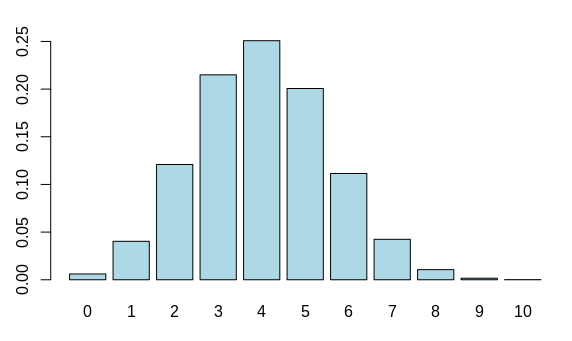
\includegraphics[width=1\linewidth]{random_distribution_binomial_1}
      \caption{Binomial p.m.f.}
    \end{minipage}
    \hfill
    \begin{minipage}{0.45\linewidth}
      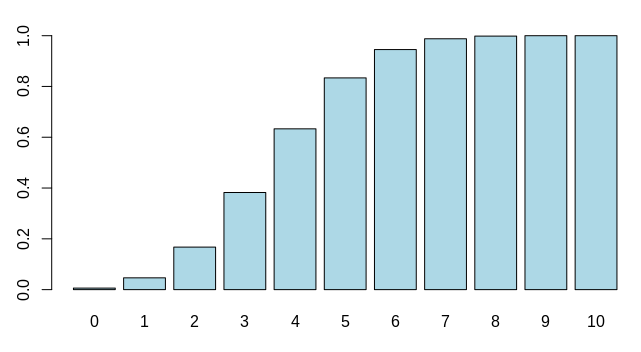
\includegraphics[width=1\linewidth]{random_distribution_binomial_2}
      \caption{Binomial c.d.f.}
    \end{minipage}
\end{figure}

\subsection{Geometric Distribution}
Consider a Bernoulli trial with probability of success $p$, the number of independent trials that result in \textit{failure} obtained before 
the first success follows a Geometric distribution with parameter $p$.
\[ X \sim \mathcal{G}(p)\]
with
\[ P(X=x) = p(1-p)^x,\;\;\; x \in \{0,1,2,\dots,n\} \]
and have expectation and variance
\[ \mathbb{E}[X] = \frac{1-p}{p},\;\;\; V[X] = \frac{1-p}{p^2} \]
\textbf{TODO.} Add base example that serves as base experiment. Ussing this base experiment we cant try to fit other rand. exp. and see
if this distribution is valid.
\begin{figure}[!ht]
    \begin{minipage}{0.45\linewidth}
      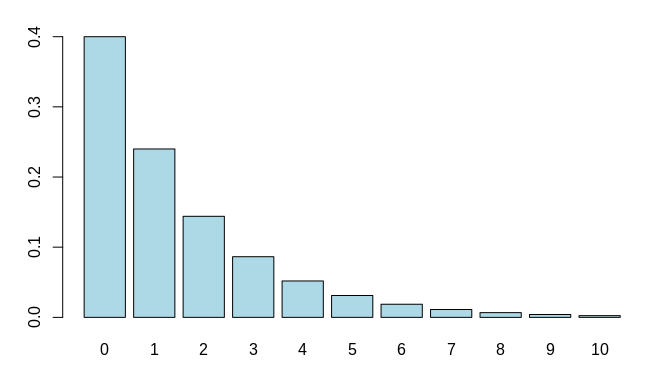
\includegraphics[width=1\linewidth]{random_distribution_geometric_1}
      \caption{Geometric p.m.f.}
    \end{minipage}
    \hfill
    \begin{minipage}{0.45\linewidth}
      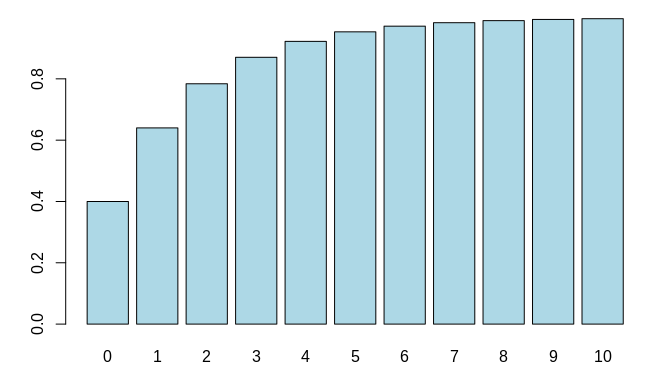
\includegraphics[width=1\linewidth]{random_distribution_geometric_2}
      \caption{Geometric c.d.f.}
    \end{minipage}
\end{figure}

\subsection{Negative Binomial Distribution}
Consider a Bernoulli trial with probability of success $p$, the number of failures (independent trials that result in failure) before the $k$-th success 
(that is, \textbf{number of trials} until $k$-success) follows a Negative Binomial distribution with parameters $k$ and $p$.
\[ X \sim NB(k,p)\]
with
\[ P(X=x) = \binom{x+k-1}{x} p^k(1-p)^x,\;\;\; x \in \{0,1,2,\dots,n\} \]
and have expectation and variance
\[ \mathbb{E}[X] = \frac{k(1-p)}{p},\;\;\; V[X] = \frac{k(1-p)}{p^2} \]

\textbf{Note: Be careful with the definition.} This distribution counts the \textbf{number of fails} not the number of fails + success\\
\textbf{TODO.} Add base example that serves as base experiment. Ussing this base experiment we cant try to fit other rand. exp. and see
if this distribution is valid.
\begin{figure}[!ht]
    \begin{minipage}{0.45\linewidth}
      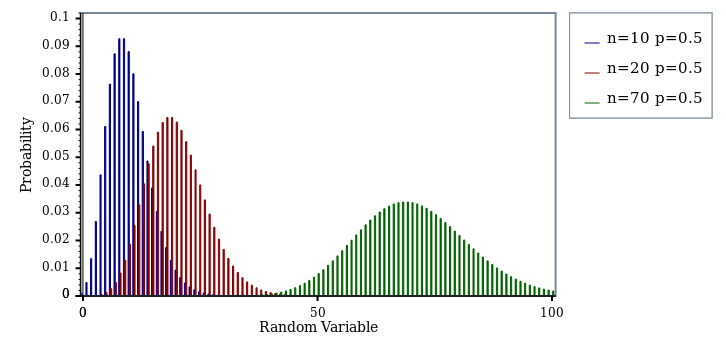
\includegraphics[width=1\linewidth]{random_distribution_negbinomial_1}
      \caption{Negative Bin. p.m.f.}
    \end{minipage}
    \hfill
    \begin{minipage}{0.45\linewidth}
      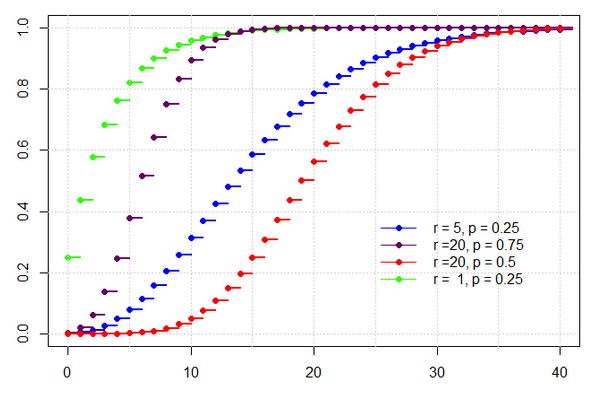
\includegraphics[width=1\linewidth]{random_distribution_negbinomial_2}
      \caption{Negative Bin. c.d.f.}
    \end{minipage}
\end{figure}

\subsection{Hypergeometric Distribution}
Consider a \textbf{finite population} with $N_1+N_2$ objects, such that $N_1$ are of type 1 and $N_2$ are of type 2. A total number of $k$
objects are selected from the population \textbf{without replacement}. The number of objects of type $N_1$ in the selection follows 
a Hypergeometric distribution with parameters $N_1, N_2$, and $k$.
\[ X \sim H(N_1,N_2,k)\]
with
\[ P(X=x) = \frac{\binom{N_1}{x}\binom{N_2}{k-x}}{\binom{N_1+N_2}{k}},\;\;\; x \in \{\max\{0,k-N_2\},\dots,\min\{k,N_1\} \} \]
and have expectation and variance
\[ \mathbb{E}[X] = \frac{kN_1}{N_1+N_2},\;\;\; V[X] = k\cdot\frac{N_1N_2}{(N_1+N_2)^2}\cdot\frac{N_1+N_2-k}{N_1+N_2-1} \]

\textbf{TODO.} Add base example that serves as base experiment. Ussing this base experiment we cant try to fit other rand. exp. and see
if this distribution is valid.
\begin{figure}[!ht]
    \begin{center}
        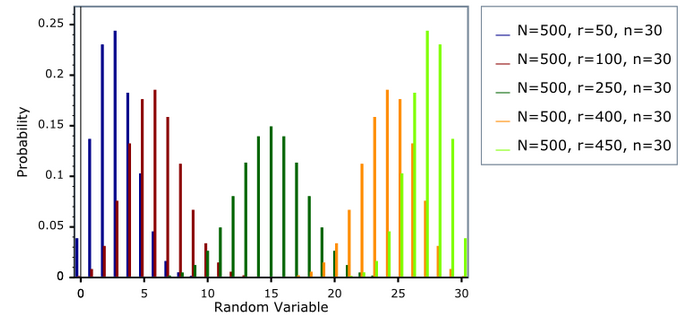
\includegraphics[width=0.4\linewidth]{random_distribution_hyperg_1}
        \caption{Hypergeometric p.m.f.}
    \end{center}
\end{figure}

\subsection{Poisson Distribution}
The number of events that occur in a region of space (or time) independently one from the others and at a constant rate $\lambda >0$ 
follows a Poisson distribution with parameter $\lambda$.
\[ X \sim \mathcal{P}(\lambda)\]
with
\[ P(X=x) = e^{-\lambda}\frac{\lambda^x}{x!},\;\;\; x \in \{0,1,2,\dots,n\} \]
and have expectation and variance
\[ \mathbb{E}[X] = \lambda,\;\;\; V[X] = \lambda \]
\textbf{TODO.} Add base example that serves as base experiment. Ussing this base experiment we cant try to fit other rand. exp. and see
if this distribution is valid.
\subsubsection{Properties}
If $X$ and $Y$ are independent, and $X \sim \mathcal{P}(\lambda_1), Y \sim \mathcal{P}(\lambda_2)$ then 
\[ X+Y \sim \mathcal{P}(\lambda_1+\lambda_2) \]

\begin{figure}[!ht]
    \begin{minipage}{0.45\linewidth}
      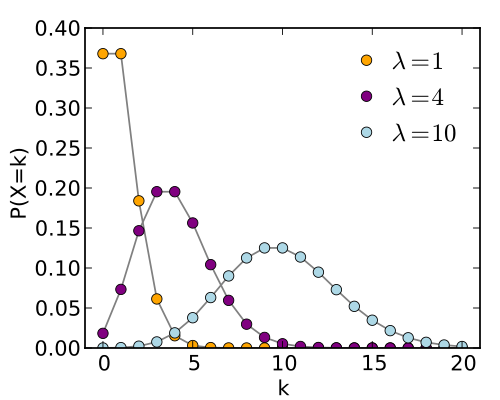
\includegraphics[width=1\linewidth]{random_distribution_poisson_1}
      \caption{Poisson p.m.f.}
    \end{minipage}
    \hfill
    \begin{minipage}{0.45\linewidth}
      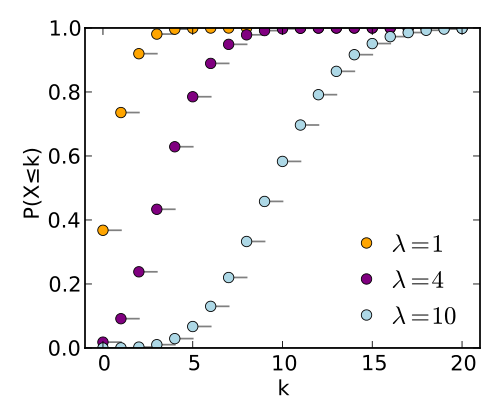
\includegraphics[width=1\linewidth]{random_distribution_poisson_2}
      \caption{Poisson c.d.f.}
    \end{minipage}
\end{figure}

\subsection{Multi Bernoulli Distribution}
TODO


\subsection{Zero Inflated Poisson Distribution}
TODO
